\chapter{SF1R Overview}
\lhead{Chapter 1. \emph{SF1R Overview}} % this is for the header on each page - perhaps a shortened title

The SF1 workflow on single machine is shown in figure\ref{fig:sf1_workflow}.
It consists of two processes. One is building process (labeled as A in the figure). The other is query process (labeled as B).

\begin{figure}[htp]
\centering
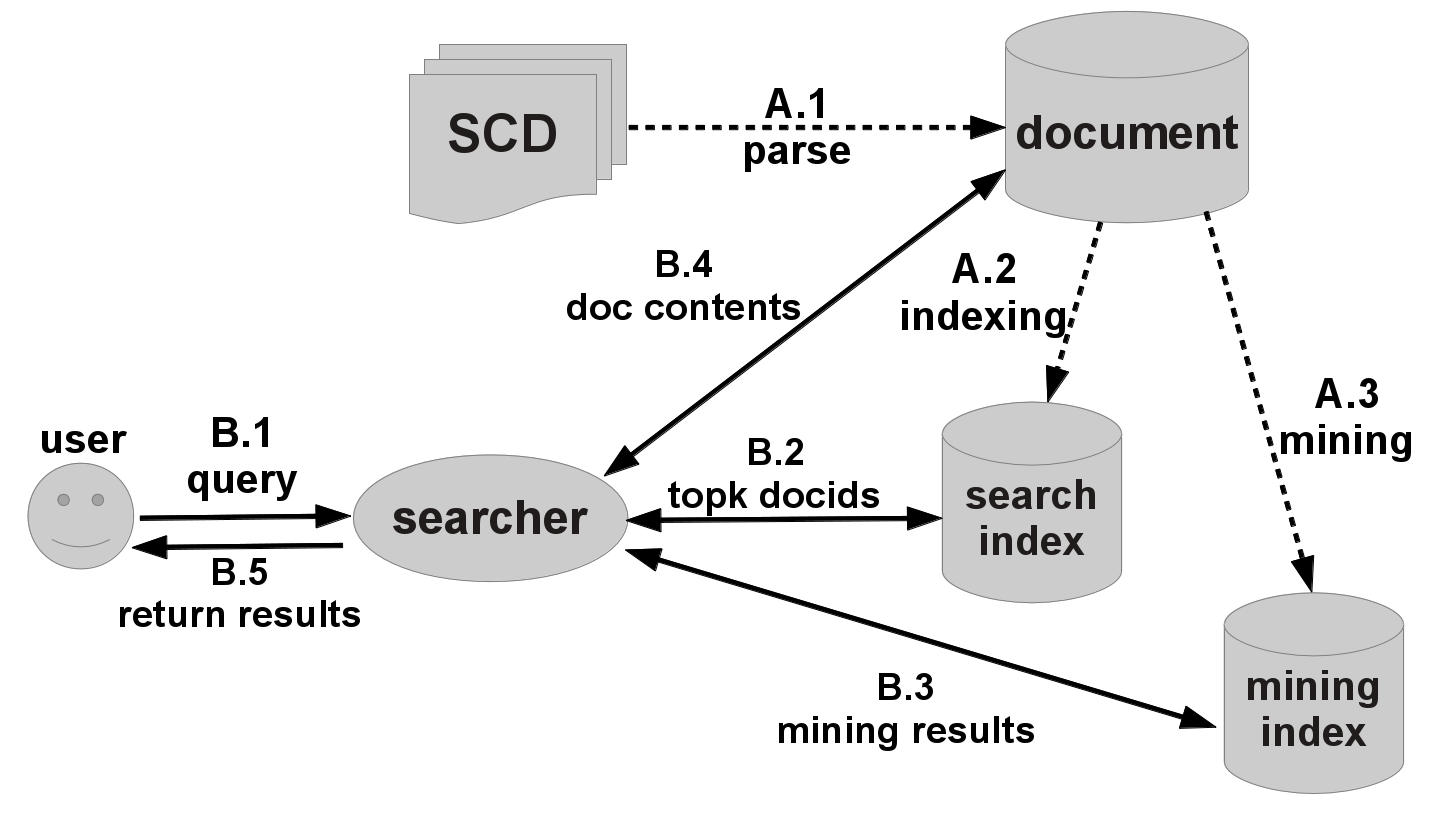
\includegraphics[width=.8\textwidth]{Figures/sf1_workflow.png}
\caption{SF1 Workflow}\label{fig:sf1_workflow}
\end{figure}

\section{Build Process}

\begin{enumerate}
\item[A.1] \textbf{SCD parsing}. The input of the building process are text files in the \textbf{SCD} format.
They are parsed into documents, and each document consists of pairs of property name and value. The documents are stored by \textbf{document manager} which
is a document oriented nosql actually.

\item[A.2] \textbf{indexing}. For those properties which are configured for search, their property values are used to build the \textbf{search index}.
To satisfy different search requirements, there are three kinds of search indices. They are \textbf{disk based index} for general search,
\textbf{suffix index} for fast fuzzy search in pure memory and \textbf{zambezi index} for fast boolean search in pure memory. For the sake of 
conveniences on implementation, \textbf{suffix index} belongs to mining procedure actually although it has the semantic of \textbf{search}. The indexing
procedure co-work with \textbf{SCD parsing} such that whenever a document is inserted into the nosql store, corresponding indices have been setup.

\item[A.3] \textbf{mining}. For those properties which are configured for mining features, such as groupby, attrby, etc,
their property values are used to build the \textbf{mining index}. \textbf{SF1R} has contained tens of mining features through \textbf{mining} procedure,
while in this technical report, only search as well as navigation relevant ones are mentioned due to frequent usage. \textbf{Mining} procedure is performed
after \textbf{indexing} stage, it directly get raw data from \textbf{document manager} and dispatch them into different kinds of mining components according
to configuration.

\end{enumerate}

\section{Query Process}

\begin{enumerate}
\item[B.1] Given the user query, it would be tokenized into \textbf{terms}.
The tokenization methods include minimum match, maximum match, maximum entropy and CRF.

\item[B.2] These terms are searched among the search index to get candidate docids.
Each candidate would be assigned with a score, calculated by ranking methods such as TF-IDF, BM25, product ranking, etc.
Finally the candidates with top scores are extracted as \textbf{topk docids}.

\item[B.3] If the request has parameters on mining features, those candidate docids are searched among the mining index to get \textbf{mining results}.

\item[B.4] The topk docids are searched among the document manager to get the \textbf{document contents}.

\item[B.5] Finally the \textbf{search results} are returned to user.

\end{enumerate}

\section{Architecture}
The architecture of \texttt{SF1R} could be seen from figure \ref{fig:sf1_architecture}, this is an overview for the system running on single machine. \texttt{SF1R}
provides unified implementation to be deployed on either single node or search cloud just via adjusting configurations. There are two separated processes within \texttt{SF1R}
system---the search engine server itself and the reverse proxy which is based on \texttt{nginx}, as shown in \ref{fig:sf1_architecture}.
\begin{figure}[htbp]
  \centering
    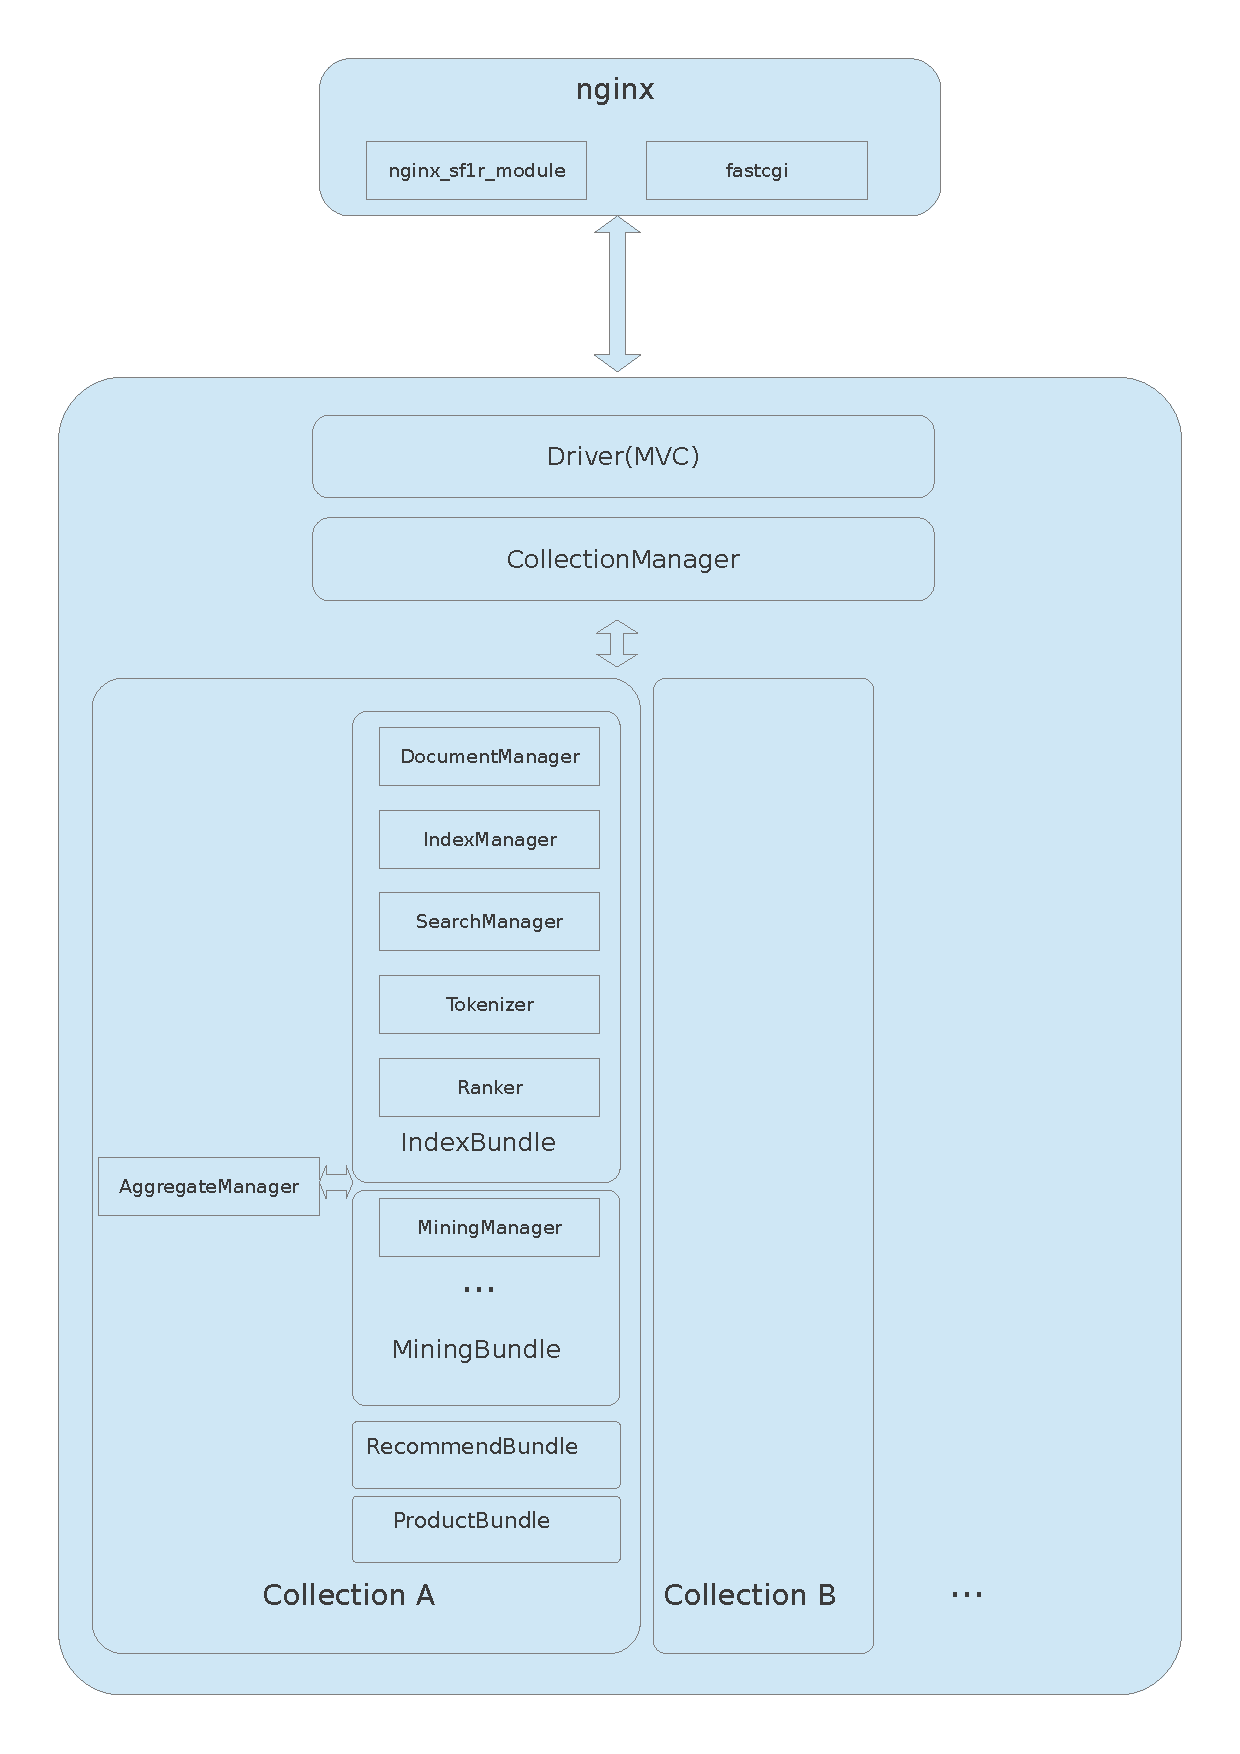
\includegraphics[width=.7\textwidth]{Figures/sf1.pdf}
    \rule{35em}{0.5pt}
  \caption[Architecture of SF1R]{Architecture of SF1R---Non-distributed On Single Machine}
  \label{fig:sf1_architecture}
\end{figure}

\subsection{Key Components}
\begin{itemize}
 \item nginx---This is the customized version to be tailed to connect with \texttt{SF1R} server, such that \texttt{http} based API could be provided to applications. As a result, 
 the client of \texttt{SF1R} is language independent. There are two kinds of mechanism for the connnection between nginx and the search engine server:
  \begin{itemize}
   \item nginx module---The nginx ecosystem delivers a flexible mechanism such that any customized module could be developed for reverse upstream servers \cite{nginx}. The nginx module runs within
   the same process together with nginx worker, as a result, when nginx is going to be connected to multiple \texttt{SF1R} servers, this is not a recommended approach for concurrency consideration.
   \item fact cgi---This is a traditional upstream mechanism for nginx ecosystem, while we have made customization to it as well such that each fast cgi process could be used to serve
   any requests routing to any remote \texttt{SF1R} server. Fast cgi is a preferred approach when deploying \texttt{SF1R} in distributed environment.
  \end{itemize}

 \item Driver---This is the network encapsulation within \texttt{SF1R} server. We borrowed the idea from web application to introduce the \texttt{MVC} pattern, such that application
 logic could be developed flexiblely based on the \texttt{Driver} layer.
 \item CollectionManager---\texttt{Collection} is the fundamental concept within \texttt{SF1R}, corresponding definition in database is \texttt{table}. The collection could be created,
 destroyed, started, as well as stopped dynamically through \texttt{CollectionManager}, just like how database manages its tables. Each request sent to \texttt{SF1R} should specify its
 target collection, such that the request could be routed correctedly.
 \item Bundle---The concept of \texttt{bundle} comes from Java enterprise community---\texttt{OSGI} \cite{osgi}. The introduction of bundle is to make the architecture more flexible and
 seperated, each collection will have its own bundle instances to make sure total separation. The existing bundles include:
  \begin{itemize}
   \item IndexBundle---It has contained core components during indexing, such as DocumentManager for data archiving, IndexManager for archive indexing,
   SearchManager and a series rankers for search operations.
   \item MiningBundle---All mining features are included in this bundle.
   \item RecommendBundle---\texttt{SF1R} has also delivered a feature to provide unified search engine and recommendation engine. RecommendBundle is for the purpose of recommendation,
   currently, the core algorithm of this engine is based on incremental item-item collaborative filtering.
  \end{itemize}
 \item AggregateManager---This is a fundamental building block for distributed search. \texttt{SF1R} provides single implementation on distributed and non-distributed version. AggregateManager
 is the key encapsulation for this unified behavior, it means, when deployed on single machine, it could be looked on as a transparent layer to serve requests, while when deployed 
 distributedly, it will have different behaviors depending on whether that node is \texttt{Master} or \texttt{Worker}:
  \begin{itemize}
   \item Worker is the node serving practical requests over its local data.
   \item Master is the node to dispatch and aggregate requests from multiple workers.
   \item Master and Worker could be deployed either together or remotely --- just via adjusting configurations.
  \end{itemize}

\end{itemize}

